%%%%%%%%%%%%%%%%%%%%%%%%%%%%%%%%%%%%%%%%%%%%%%%%%%%%%%%%%%%%%%%%%%%%%%%%%%%%%%%
\chapter{Calor Específico de Sólidos} % Sem "Experiência 01" ou qualquer outro número
\label{Chap:CalorEspecifico}        % para poder trocar a ordem com facilidade
%%%%%%%%%%%%%%%%%%%%%%%%%%%%%%%%%%%%%%%%%%%%%%%%%%%%%%%%%%%%%%%%%%%%%%%%%%%%%%%

\begin{fullwidth}\it
Verificaremos o calor específico de alguns materiais, buscando comprovar experimentalmente as trocas energéticas envolvidas em transferências de calor. Veremos também a explicação para os fenômenos observados segundo a Primeira Lei da Termodinâmica. Utilizaremos os seguintes conceitos/técnicas de análise de dados: medidas, algarismos significativos, gráficos, software para elaboração de gráficos, erros de escala e propagados, equação geral para o erro propagado, regressão linear, linearização, erros dos coeficientes $A$ e $B$, e planílhas para cálculo dos coeficientes $A$ e $B$ com erros.
\end{fullwidth}

%%%%%%%%%%%%%%%%%%%%%%%%%%%%%%%%%%%%%%%%%%%%%%%%%%%%%%%%%%%%%%%%%%%%%%%%%%%%%%%
\section{Princípio da conservação da energia}
%%%%%%%%%%%%%%%%%%%%%%%%%%%%%%%%%%%%%%%%%%%%%%%%%%%%%%%%%%%%%%%%%%%%%%%%%%%%%%%

%Exp. acontece no início do estudo de termodinâmica, por isso precisamos explicar o que é calor do ponto de vista de energia. Pra isso precisamos falar sobre trabalho e primeira lei da termodinâmica.

%Começar falando do calórico e da observação do Rumford ao perfurar os canhões

%Falar da Lei Zero da Termo.
%Falar sobre os processos de condução de calor e sobre a variação da energia interna e sua relação com a variação da temperatura/interpretação microscópica da temperatura.

%Falar sobre a determinação do equivalente mecânico para o calor

%O calor é armazenado como energia interna se $W=0$. Isso se reflete em uma mudanção na temperatura. No entanto, substâncias diferentes têm calores específicos diferentes. Por quê?
%Ver explicação do armazenamento de energia para um gás monoatômico e diatômico. Falar que o calor específico não é constante, que depende dos modos energéticos ativados. E que obviamente depende da fase do objeto (pq? deve ser pq mudam os modos de armazenamento de energia disponíveis)
%Ver sobre origens do calor específico dos sólidos.

Sabemos que a soma da energia cinética e da energia potencial de um sistema dá origem ao que denominamos como \emph{energia mecânica}:
\begin{align}
    E &= K + \sum U \\
    &= \frac{mv^2}{2} + \left(mgy + \frac{kx^2}{2} + \dots\right).
\end{align}
%
Se em um sistema qualquer atuam somente \emph{forças conservativas}, a energia mecânica será constante. Se existe uma \emph{força não-conservativa}, no entanto, temos que
\begin{equation}\label{Eq:TrabalhoNCIgualVarEnergiaMec}
    \Delta E^{\text{mec}} = W_{\text{NC}}.
\end{equation}
% 
Vamos considerar agora o que acontece com a energia em duas situações diferentes, ambas sujeitas a atuação de uma força não-conservativa. 

\begin{marginfigure}
\centering
\begin{tikzpicture}[>=Stealth,
     interface/.style={
        % superfície
        postaction={draw,decorate,decoration={border,angle=-45,
                    amplitude=0.2cm,segment length=2mm}}},
    ]
    
    \draw[interface] (-2,0) -- (2,0);
    
    \draw[pattern = north west lines] (-0.1, 1.4) -- (-0.1,1.2) -- (-0.5, 1.2) -- (-0.5, 0.2) -- (0.5, 0.2) -- (0.5, 1.2) -- (0.1, 1.2) -- (0.1,1.4) -- (0.7,1.4) -- (0.7,0) -- (-0.7,0) -- (-0.7, 1.4) -- cycle;
    
    \draw[pattern = north east lines] (-0.4, 0.55) -- (-0.4, 0.45) -- (0.4, 0.45) -- (0.4, 0.55) -- (0.05, 0.55) -- (0.05, 2) -- (-0.05, 2) -- (-0.05, 0.55) -- cycle;
    
    \fill[pattern = dots] (-0.5, 0.2) rectangle (0.5, 1.2);
    
    \draw[pattern = north west lines] (-0.5, 2) rectangle (0.5, 3);
       
    \draw[decoration={aspect=0.5, segment length=1mm, amplitude=1mm,coil},decorate] (0,3) -- (0,4);
    
    \draw[interface] (2,4) -- (-2,4);
    
    \draw[dashed] (-2.2, 4.5) rectangle (2.2, 1.7); 

    
\end{tikzpicture}
\caption{Bloco suspenso por uma mola, livre para oscilar, porém conectado a um sistema de amortecimento.\label{Fig:OsciladorAmortecido}}
\end{marginfigure}

Primeiramente, vamos considerar um bloco suspenso por uma mola e livre para oscilar. Na parte inferior do bloco, existe uma haste que está fixada a ele e cuja extremidade oposta está ligada a uma placa plana, submersa em água ---~veja a Figura~\ref{Fig:OsciladorAmortecido}~---. Sabemos que o deslocamento da placa dentro do fluido está sujeito a uma força de arrasto, sempre na direção contrária ao seu deslocamento. Isso implica em uma força que atua sobre o bloco através da haste, realizando trabalho negativo, fazendo com que sua energia mecânica seja diminuida a cada oscilação:
\begin{align}
    \Delta E^{\text{mec}} &= W_{\text{NC}} \\
    &= W_{F_{\text{haste}}}.
\end{align}
%
Eventualmente, o movimento oscilatório cessará devido ao fato de que a energia mecânica se tornará nula. Se considerarmos o sistema formado somente pelo bloco e pela mola, podemos dizer que há uma \emph{força externa} ---~a força exercida pela haste~--- que diminui a energia mecânica do sistema. Por outro lado, verificamos também que tal força exerce um trabalho \emph{positivo} sobre o fluido, forçando-o a se movimentar. Dessa forma, podemos dizer que o trabalho de uma força externa \emph{transfere} a energia através da fronteira do sistema (representada na figura pelo retângulo tracejado).\footnote{Sabemos que pelo menos uma parte da energia é transferida para o fluido, manifestando-se como energia cinética.}

Vamos supor agora que temos um sistema onde atuam forças conservativas e uma força não-conservativa \emph{interna}, ou seja, uma força cujo par ação-reação esteja completamente contido dentro da fronteira do sistema. Um exemplo desse caso pode ser uma força de atrito entre um bloco e uma superfície em um sistema como o mostrado na Figura~\ref{Fig:MassaMolaSistemaFechado}. Vamos assumir que nenhuma força externa \emph{que realize trabalho} atue sobre tal sistema, atravessando sua fronteira ---~vamos desconsiderar efeitos da força de arrasto; a força normal que atua sobre o sistema é externa, porém seu trabalho é nulo~---. Nessa situação, verificamos que se aplica a expressão
\begin{align}
    \Delta E_S &= W_{\text{NC}} \\
    &= W_{\text{at}}.
\end{align}

\begin{marginfigure}
\centering
\begin{tikzpicture}[>=Stealth, scale = 0.75,
     interface/.style={
        % superfície
        postaction={draw,decorate,decoration={border,angle=-45,
                    amplitude=0.2cm,segment length=2mm}}},
    ]
      
    \draw[pattern = north east lines] (0,-1.5) -- (0,-3) -- (4.8, -3) -- (4.8, -3.4) -- (-0.5,-3.4) -- (-0.5,-1.5) -- cycle;
    
    \draw (0,-2.5) -- (0.2,-2.5);
    \draw[decoration={aspect=0.3, segment length=2.5625mm, amplitude=2mm,coil},decorate] (0.2,-2.5) -- (3.3,-2.5);
    \draw (3.3, -2.5) -- (3.5,-2.5);
    
    \draw[interface] (-0.7, -3.4) -- (5, -3.4);
    
    \draw[pattern = north west lines] (3.5,-3) rectangle (4.5,-2);
    
    \draw[dashed] (-1, -1) rectangle (5.3, -3.9);
        
\end{tikzpicture}
\caption{Sistema formado por um oscilador massa-mola sujeito a uma força de atrito. Se nenhuma força que atravessa a fronteira do sistema realiza trabalho, então o sistema é \emph{fechado}.\label{Fig:MassaMolaSistemaFechado}}
\end{marginfigure}

Segundo a equação acima, a energia mecânica deve diminuir, porém estamos considerando um \emph{sistema fechado}, ou seja, não pode haver fluxo de energia através da fronteira. Nesse momento, aparentemente deveríamos argumentar que a energia se perdeu, afinal, estamos tratando de uma situação em que atua uma força não-conservativa. Essa ideia, porém, não descreve o que acontece quando uma força não conservativa atua de maneira a realizar trabalho através da fronteira, como no caso da força exercida pela haste no exemplo anterior. Além disso, é comum em situações como a da Figura~\ref{Fig:MassaMolaSistemaFechado} que se note um \emph{aumento da temperatura do sistema}, isto é, um aumento da temperatura do bloco e da superfície onde ele se apoia.

\begin{marginfigure}
\centering
\begin{tikzpicture}[>=Stealth, scale = 1,
     interface/.style={
        % superfície
        postaction={draw,decorate,decoration={border,angle=-45,
                    amplitude=0.2cm,segment length=2mm}}},
    ]
      

    \draw[interface] (-0.05,1.35) -- (-0.05,-0.05) -- (4,-0.05) -- (4,1.35);
    
    \draw (-0.05,0.5) -- (0.2,0.5);
    \draw[decoration={aspect=0.3, segment length=1.1mm, amplitude=2mm,coil},decorate] (0.2,0.5) -- (2,0.5);
    \draw (2,0.5) -- (3,0.5);
    
    \draw[pattern = crosshatch] (3,0.15) rectangle (3.15, 0.85);
    
    \draw[pattern = north west lines] (2.5,0.15) -- (2.5,-0.05) -- (4, -0.05) -- (4,1.05) -- (2.5,1.05) -- (2.5,0.85) -- (3.8, 0.85) -- (3.8, 0.15) -- cycle;
    \path[pattern = dots] (3.15,0.15) rectangle (3.8,0.85);
    
    \draw[dashed] (-0.55, -0.55) rectangle (4.5,1.85);
    
\end{tikzpicture}
\caption{No sistema acima, a mola inicialmente armazena energia potencial elástica. Ao a liberarmos para que se mova, a energia mecânica sofre uma variação devido ao trabalho exercido através da haste sobre o gás.\label{Fig:PistaoEMola}}
\end{marginfigure}

Outro sistema que apresenta uma comportamento similar ao do sistema massa-mola da Figura~\ref{Fig:MassaMolaSistemaFechado} é o mostrado na Figura~\ref{Fig:PistaoEMola}, onde uma mola está inicialmente comprimida e está ligada a um êmbolo que pode comprimir um gás. Ao liberarmos a mola para que se expanda, verificamos uma diminuição da energia mecânica devido ao trabalho exercido sobre a mola pelo gás, através da haste. No entanto, como nenhuma força que atravessa a fronteira do sistema realiza trabalho, novamente temos uma aparente perda da energia. Mais uma vez, notamos um aumento da temperatura do sistema: ao comprimirmos o gás, sua temperatura aumenta. Se, por outro lado, aumentarmos a temperatura do gás utilizando a chama de uma vela, por exemplo, vamos notar algo interessante: o gás se expande, comprimindo a mola. Ou seja, verificamos um aumento da energia mecânica do sistema. Percebemos assim que \emph{a temperatura está ligada a uma outra forma de energia}.

Nos sistemas das Figuras~\ref{Fig:MassaMolaSistemaFechado} e~\ref{Fig:PistaoEMola} concluímos que a energia mecânica deve ter sido transformada em algum outro tipo de energia, que denominamos como \emph{energia interna}, e que está relacionada à temperatura do corpo\footnote[][-3cm]{Microscopicamente, a energia interna associada à temperatura de um corpo está relacionada à velocidade média das partículas que o compõe: no caso da Figura~\ref{Fig:PistaoEMola}, para que o gás comprima a mola ao ter sua temperatura aumentada devido à chama da vela, verificamos que a força média exercida pela colisão das moléculas do gás sobre a parede do êmbolo só pode aumentar se o número de partículas no cilindro, a massa das moléculas, ou as velocidades das moléculas aumentarem. Como os dois primeiros fatores são constantes, concluímos que a velocidade das moléculas aumenta com a temperatura.}. Logo, podemos somar a variação da energia mecânica à variação da energia interna de um sistema e escrever
\begin{equation}\label{Eq:ConservacaoDaEnergia1}
    \Delta E_S^{\text{mec}} + \Delta E_S^{\text{int}} = W_{F_{\text{ext}}},
\end{equation}
%
onde $W_{F_{\text{ext}}}$ representa o trabalho total efetuado por forças que atravessam a fronteira do sistema. Note que a expressão acima assume o caráter de uma \emph{lei de conservação} para a energia do sistema, uma vez que só é possível alterá-la através do trabalho de uma força externa ---~ isto é, de uma força que cruza a fronteira do sistema e que realize trabalho~---.

%%%%%%%%%%%%%%%%%%
\subsection{Calor}
%%%%%%%%%%%%%%%%%%

\begin{marginfigure}
\centering
\begin{tikzpicture}[>=Stealth, scale = 1,
     interface/.style={
        % superfície
        postaction={draw,decorate,decoration={border,angle=-45,
                    amplitude=0.2cm,segment length=2mm}}},
    ]
      
    \draw[interface] (0,0) -- (4.5,0);
    
    \draw[pattern = north west lines] (2.5,0) rectangle +(1,1);
    \draw[draw=black, fill=white] (3,0.5) circle (2.5mm) node{$T_2$};
    
    \node (a) at (2.25, 1.25) {$T_1 > T_2$};
    
    \draw[pattern = north east lines] (2,0) rectangle +(-1,1);
    \draw[draw=black, fill=white] (1.5,0.5) circle (2.5mm) node {$T_1$};
    
    \begin{scope}[shift={(0,-2)}]
        \draw[interface] (0,0) -- (4.5,0);
    
        \draw[pattern = north west lines] (2.25,0) rectangle +(1,1);
        \draw[draw=black, fill=white] (2.75,0.5) circle (2.5mm) node{$T_2$};
    
        \draw[pattern = north east lines] (2.25,0) rectangle +(-1,1);
        \draw[draw=black, fill=white] (1.75,0.5) circle (2.5mm) node {$T_1$};
        
        \draw[->] (2,1.25) -- node[above]{$Q$} (2.75,1.25);
    \end{scope}
    
    \begin{scope}[shift={(0,-4)}]
        \draw[interface] (0,0) -- (4.5,0);
    
        \draw[pattern = north west lines] (2.25,0) rectangle +(1,1);
        \draw[draw=black, fill=white] (2.75,0.5) circle (2.5mm) node{$T_2$};
    
        \draw[pattern = north east lines] (2.25,0) rectangle +(-1,1);
        \draw[draw=black, fill=white] (1.75,0.5) circle (2.5mm) node {$T_1$};
        
        \node (b) at (2.25,1.25) {$T_1 = T_2 = T_{\text{eq}}$};
    \end{scope}
    
    \begin{scope}[shift={(0,-6)}]
        \draw[interface] (0,0) -- (4.5,0);
    
        \draw[pattern = north west lines] (2.5,0) rectangle +(1,1);
        \draw[draw=black, fill=white] (3,0.5) circle (2.5mm) node{$T_{\text{eq}}$};
    
        \draw[pattern = north east lines] (2,0) rectangle +(-1,1);
        \draw[draw=black, fill=white] (1.5,0.5) circle (2.5mm) node {$T_{\text{eq}}$};
        
%        \node (b) at (2.25,1.25) {$T_1 = T_2 = T_{\text{eq}}$};
    \end{scope}
\end{tikzpicture}
\caption{Se dois blocos a temperaturas diferentes são postos em contato, existe uma fluxo de energia interna entre eles que tende a equilibrar suas temperaturas.}
\end{marginfigure}

Se a energia interna está associada à temperatura, então existe uma maneira de transferir energia para fora de um sistema que não envolve a realização de trabalho por uma força externa: se tomarmos dois sistemas distintos ---~ como, por exemplo, dois blocos metálicos~--- a temperaturas diferentes, é fácil perceber que ao deixarmos que ambos fiquem em contato direto a temperatura do bloco frio aumenta e a temperatura do bloco quente diminui. A tal fluxo de energia interna denominamos \emph{calor}\footnote{Microscopicamente, como a temperatura dos blocos é diferente, a energia cinética média das partículas que compõe cada um deles também são diferentes. No contato direto entre ambos, as partículas do corpo quente interagem com as do corpo frio, forçando-as a oscilar. Ocorre uma transferência de energia cinética entre as partículas de cada um dos corpos através do trabalho das forças entre as cargas elétricas dos átomos.}. Devemos então adicionar um termo $Q$ à direita da Expressão~\eqref{Eq:ConservacaoDaEnergia1}, relativo ao calor transmitido:
    \begin{equation}\label{Eq:ConservacaoDaEnergia1Q}
    \Delta E_S^{\text{mec}} + \Delta E_S^{\text{int}} = W_{F_{\text{ext}}} + Q.
\end{equation}


%%%%%%%%%%%%%%%%%%%%%%%%%%%%%%%%%%%%%%%%%%%%%%%
\subsection{Outras formas de energia, radiação}
%%%%%%%%%%%%%%%%%%%%%%%%%%%%%%%%%%%%%%%%%%%%%%%

Apesar de a expressão acima ser mais geral que a Expressão~\eqref{Eq:TrabalhoNCIgualVarEnergiaMec}, ainda podemos imaginar uma série de possibilidades que não são bem descritas por ela:
\begin{description}
    \item[Energia química:] Se, por exemplo, utilizarmos um motor elétrico ligado a uma bateria, sabemos que é possível o utilizar para alterar a energia mecânica do sistema, mesmo sem a ação de uma força externa. De fato, existe uma \emph{energia química} armazenada na bateria que nos permite utilizar o trabalho da força não-conservativa exercida pelo motor para fazer variar a energia mecânica do sistema, ou a energia interna do sistema, ou mesmo ambas. Outra possibilidade é a de utilizar um combustível e substituir o motor elétrico por uma máquina térmica: assim como no caso da bateria, os combustíveis são uma maneira de armazenar energia química. Como esse tipo de energia tem um caráter similar à energia interna associada à temperatura, não há necessidade de alterar a Expressão~\eqref{Eq:ConservacaoDaEnergia1}.\footnote{Microscopicamente, a energia química é uma energia potencial elétrica armazenada nas configurações moleculares dos átomos.}

    \item[Radiação eletromagnética:] Sabemos que o Sol é capaz de causar variações de temperatura na Terra, mesmo na ausência de um \emph{meio de contato} entre ambos. Devido à ausência de tal meio, não é possível que haja transmissão de energia interna através de um fluxo de calor. Também não existe uma força que atravesse ambas as fronteiras, realizando trabalho\footnote{Na verdade, a força gravitacional entre o Sol e a Terra, ou entre a Lua e a Terra, pode realizar trabalho: essa é a origem das marés. A quantidade de energia transmitida, no entanto, é muito menor que através da radiação.}. Resta então a transmissão de energia através de \emph{radiação eletromagnética}. A radiação eletromagnética, é uma perturbação de caráter ondulatório nos campos elétrico e magnético que preenchem o espaço, e também é conhecida como \emph{ondas eletromagnéticas}. Como tais campos podem existir mesmo no vácuo, as ondas eletromagnéticas podem se propagar na ausência de matéria. Representamos a radiação eletromagnética através de um termo $R$ à direita da Expressão~\eqref{Eq:ConservacaoDaEnergia1}.
\end{description}
 
Considerando as observações acima, podemos \emph{postular} um \emph{princípio de conservação da energia}:
\begin{equation}\label{Eq:ConservacaoDaEnergia2}
    \Delta E_S^{\text{mec}} + \Delta E_S^{\text{int}} = W_{F_{\text{ext}}} + Q + R. \mathnote{Princípio da conservação da energia (1\textordfeminine~Lei da Termodinâmica)}
\end{equation}
%
Tal expressão é um postulado pois não é possível prová-la: verificamos nos exemplos discutidos acima que existem indícios de que a energia é transmitida entre sistemas diferentes, através de diferentes meios, porém não é possível verificar/provar que nenhuma parte da energia é perdida. No entanto, todas as evidências experimentais levam a crer que o princípio acima é válido.\footnote{Ao se realizar um experimento, é muito comum que parte da energia seja \emph{dissipada} em outras formas. No entanto, se mensurarmos a quantidade de energia dissipada, ou alterarmos o aparato experimental de maneira a minimizar a perda energética, verificamos que a Equação~\eqref{Eq:ConservacaoDaEnergia2} é sempre satisfeita. Isso, porém, é na prática extremamente difícil.}

Através do princípio da conservação da energia e da flexibilidade que temos ao definir um sistema, podemos nos preocupar simplesmente com o \emph{fluxo} da energia. Isso tende a facilitar muito a interpretação de diversos problemas pois podemos nos preocupar com a origem e o destino da energia, sem nos atermos a cada detalhe dos processos físicos que ocorrem durante a transferência da energia entre uma forma e outra.


%%%%%%%%%%%%%%%%%%%%%%%%%%%%%%%%%%%%%%%%%%
\section{Calor Específico}
%%%%%%%%%%%%%%%%%%%%%%%%%%%%%%%%%%%%%%%%%%

\begin{marginfigure}[1cm]
\centering
\begin{tikzpicture}[>=Stealth, scale = 1,
     interface/.style={
        % superfície
        postaction={draw,decorate,decoration={border,angle=-45,
                    amplitude=0.2cm,segment length=2mm}}},
    ]
      
    \draw[interface] (0,0) -- (4.5,0);
    
    \draw[pattern = north west lines] (2.5,0) rectangle +(1,1);
    \draw[draw=black, fill=white] (3,0.5) circle (2.5mm) node{$T_i$};
    
    \draw[pattern = crosshatch] (2,0) rectangle +(-1,1);
    \draw[draw=black, fill=white] (1.5,0.5) circle (2.5mm) node {$Q$};
    
    \begin{scope}[shift={(0,-2)}]
        \draw[interface] (0,0) -- (4.5,0);
    
        \draw[pattern = north west lines] (2.5,0) rectangle +(1,1);
        \draw[draw=black, fill=white] (3,0.5) circle (2.5mm) node{$T$};
    
        \draw[pattern = crosshatch] (2.5,0) rectangle +(-1,1);
        \draw[draw=black, fill=white] (2,0.5) circle (2.5mm) node {$Q$};
    \end{scope}
    
    \begin{scope}[shift={(0,-4)}]
        \draw[interface] (0,0) -- (4.5,0);
    
        \draw[pattern = north west lines] (2.5,0) rectangle +(1,1);
        \draw[draw=black, fill=white] (3,0.5) circle (2.5mm) node{$T_f$};
    
        \draw[pattern = crosshatch] (2,0) rectangle +(-1,1);
        \draw[draw=black, fill=white] (1.5,0.5) circle (2.5mm) node {$Q$};
    \end{scope}
\end{tikzpicture}
\caption{Um corpo entra em contato com uma fonte térmica, sofrendo uma variação em sua temperatura.\label{Fig:BlocoContatoFonteCalor}}
\end{marginfigure}

Vamos considerar um corpo qualquer que repousa sobre uma mesa e pode ser posto em contato com um uma fonte de calor (Figura~\ref{Fig:BlocoContatoFonteCalor}). Se a fonte ceder uma certa quantidade de calor, podemos determinar a variação de energia interna através do princípio de conservação da energia. Obtemos então
\begin{align}
    \Delta E^{\text{mec}} + \Delta E^{\text{int}} &= W_{\text{ext}} + Q \\
    \Delta E^{\text{int}} &= Q,
\end{align}
%
onde $\Delta E^{\text{mec}}$ é zero pois não há variação nem da energia cinética, nem de qualquer energia potencial. Além disso, não existe nenhum trabalho efetuado sobre o corpo, portanto $W_{\text{ext}}$ também é zero.

Nessas condições, é possível verificar experimentalmente que 
\begin{align}
    Q &= \Delta E^{\text{int}} \\
    &= m c \Delta T,
\end{align}
%
onde $m$ representa a massa do corpo, $c$ é uma constante característica do material de que o corpo é feito ---~denominada \emph{calor específico}~---, e $\Delta T$ representa a variação de temperatura do corpo.

\begin{margintable}[-1cm]
\begin{tabular}{ccc}
	\toprule
	Material & $\rm{J/kg\cdot\tcdegree C}$ & $\rm{cal/g\cdot\tcdegree C}$ \\
	\midrule
	Alumínio & 900 & \np{0,215} \\
	Cobre & 387 & \np{0,0924} \\
	Ferro & 448 & \np{0,107} \\
	Chumbo & 128 & \np{0,0305} \\
	Latão & 380 & \np{0,092} \\
	Água & 4186 & \np{1,00} \\
	\bottomrule
\end{tabular}
\vspace{1mm}
\caption{Calor específico para alguns materiais à temperatura de \np[\tcdegree C]{25}. \label{Tab:CaloresEspecificosDeReferencia}% Tirei do Serway, talvez fosse melhor arranjar uma referência melhor, de alguém que medisse o treco e colocasse o erro pelo menos.
}
\end{margintable}

%%%%%%%%%%%%%%%%%%%%%%%%%%%%%%%
\subsection{Capacidade Térmica}
%%%%%%%%%%%%%%%%%%%%%%%%%%%%%%%

Em muitas situações temos corpos que não são feitos de um único material. Nesse caso, podemos relacionar o calor transferido para o corpo e a consequente variação da temperatura através da \emph{capacidade térmica} $C$, de forma que
\begin{align}
    Q &= \Delta E^{\text{int}} \\
    &= C \Delta T.
\end{align}
%
Note que para um corpo constituido de um único tipo de material, podemos relacionar a capacidade térmica e o calor específico através de
\begin{equation}
    C = m c.
\end{equation}

%%%%%%%%%%%%%%%%%%%%%%%%%%%%%%%%%%%%%%%%%%%%%%%%%%%%%%%%%%%%%%%%%
\subsection{Determinação da Capacidade Térmica de um Calorímetro}
%%%%%%%%%%%%%%%%%%%%%%%%%%%%%%%%%%%%%%%%%%%%%%%%%%%%%%%%%%%%%%%%%

Para que possamos determinar o calor específico utilizando um calorímetro, devemos antes de tudo determinar qual é a quantidade de calor que será absorvida pelo próprio calorímetro. Se inicialmente temos o calorímetro e dentro dele uma massa de água fria $m_{\text{fria}}^{\text{água}}$, sendo que ambos se encontram em equilíbrio térmico a uma temperatura $T_i$, ao adicionarmos uma massa $m_{\text{quente}}^{\text{água}}$ de água quente, a uma temperatura $T_q$, obteremos uma temperatura final $T_f$. Analisando as trocas de calor, verificamos que
\begin{align}
    \Delta E_S^{\text{mec}} + \Delta E_S^{\text{int}} &= W_{F_{\text{ext}}} + Q + R \\
    \Delta E_S^{\text{int}} &= 0,
\end{align}
%
onde verificamos que não ocorrem variações de energia mecânica apreciáveis e também que não temos trocas de calor, radiação, ou trabalho de forças externas entre o calorímetro e o ambiente. Apesar de a energia interna total do sistema também não variar, a energia interna de cada componente pode variar independentemente, logo
\begin{equation}
    \Delta E_{\text{água quente}}^{\text{int}} + \Delta E_{\text{água fria}}^{\text{int}} + \Delta E_{\text{calorímetro}}^{\text{int}} = 0.
\end{equation}
%
Tais variações de energia interna se devem ao calor que flui entre os componentes do sistema, de forma que
\begin{equation}
	Q^{\text{água quente}}_{\text{perdido}} + Q^{\text{água fria}}_{\text{ganho}} + Q^{\text{Calorímetro}}_{\text{ganho}} = 0.
\end{equation}
%
Logo, se substituirmos $Q = mc\Delta T$ para o calor ganho ou perdido pela água e $Q = C\Delta T$ para o calor ganho pelo calorímetro\footnote{As constante $c$ e $C$ representam o calor específico da água e a capacidade térmica do calorímetro, respectivamente.}, temos
\begin{equation}
	m_{\text{quente}}^{\text{água}} c (T_f - T_q) + m_{\text{fria}}^{\text{água}} c (T_f - T_i) + C(T_f - T_i) = 0,
\end{equation}
%
de onde obtemos
\begin{equation}
	C = -c\cdot\left[\frac{m_{\text{quente}}^{\text{água}}(T_f - T_q)+m_{\text{fria}}^{\text{água}}(T_f - T_i)}{(T_f - T_i)}\right].
\end{equation}

%%%%%%%%%%%%%%%%%%%%%%%%%%%%%%%%%%%%%%%%%%%%%
\subsection{Determinação do Calor Específico}
%%%%%%%%%%%%%%%%%%%%%%%%%%%%%%%%%%%%%%%%%%%%%

Para determinar o calor específico devemos tomar o calorímetro com uma massa $m$ de água fria, ambos em equilíbrio térmico a uma temperatura inicial $T_i$. Se tomarmos uma amostra aquecida a uma temperatura $T_q$ e a adicionarmos ao calorímetro, temos após o equilíbrio uma temperatura final $T_f$. Analisando as trocas de calor obtemos
\begin{align}
    \Delta E_S^{\text{mec}} + \Delta E_S^{\text{int}} &= W_{F_{\text{ext}}} + Q + R \\
    \Delta E_S^{\text{int}} &= 0,
\end{align}

\begin{marginfigure}[2cm]
	\centering
	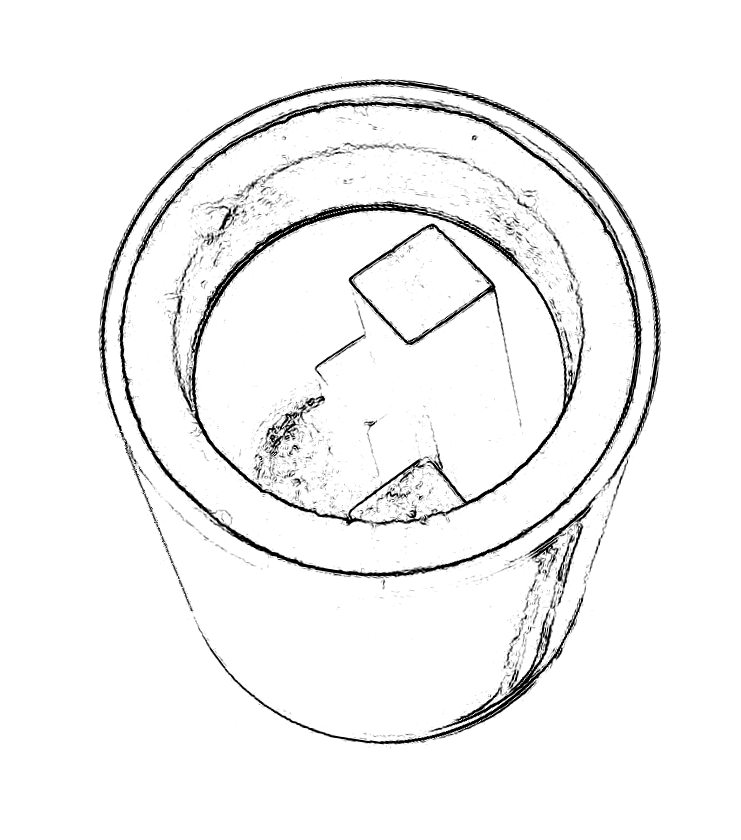
\includegraphics[width=0.8\textwidth]{Ilustrations/Calorimetro.png}
	\caption{Calorímetro aberto.}
\end{marginfigure}

\noindent{}onde novamente temos que não ocorrem variações de energia mecânica apreciáveis e também que não temos trocas de calor, radiação, ou trabalho de forças externas entre o calorímetro e o ambiente. Como a energia interna de cada componente pode variar independentemente,
\begin{equation}
    \Delta E_{\text{água quente}}^{\text{int}} + \Delta E_{\text{água fria}}^{\text{int}} + \Delta E_{\text{calorímetro}}^{\text{int}} = 0,
\end{equation}
%
o que resulta em
\begin{equation}
	Q^{\text{Corpo}}_{\text{perdido}} + Q^{\text{água}}_{\text{ganho}} + Q^{\text{Calorímetro}}_{\text{ganho}} = 0
\end{equation}
%
Substituindo as expressões $Q = m c \Delta T$ para o ganho de calor pela água, $Q = m_a c_a \Delta T$ para o calor perdido pela amostra, e $Q = C\Delta T$ para o calor ganho pelo calorímetro, temos
\begin{equation}
	m_a c_a (T_f - T_q) + m c (T_f - T_i) + C (T_f-T_i) = 0.
\end{equation}
%
Obtemos então para o calor específico da amostra
\begin{equation}
	c_a = - \left[\frac{(mc + C)\cdot(T_f - T_i)}{m_a (T_f - T_q)}\right]
\end{equation}

%%%%%%%%%%%%%%%%%%%%%%%%%%%%%%%%%%%%%%%%%%%%%%%%%%%%%%%%%%%%%%%%%%%%%%%%%%%%%%%
\section{Experimento}
%%%%%%%%%%%%%%%%%%%%%%%%%%%%%%%%%%%%%%%%%%%%%%%%%%%%%%%%%%%%%%%%%%%%%%%%%%%%%%%

Vamos utilizar o Princípio da conservação da energia para determinar a capacidade térmica de um calorímetro. Para isso, basta adicionarmos ao calorímetro água quente a uma temperatura conhecida e verificar o ganho de massa do sistema e sua temperatura final. Após isso, podemos adicionar ao calorímetro corpos diversos ---~um de cada vez~---, aferindo a temperatura e a massa finais do sistema. Utilizando o Princípio da Conservação da Energia mais uma vez, determinaremos o calor específico dos sólidos em questão.

%%%%%%%%%%%%%%%%%%%%%%
\subsection{Objetivos}
\label{Sec:ObjetivosCalorEspecifico}
%%%%%%%%%%%%%%%%%%%%%%

\begin{enumerate}
	\item Determinar experimentalmente o calor específicos de diferentes materiais sólidos;
	\item Observar o equilíbrio térmico entre os corpos;
	\item Observar a validade da Primeira Lei da Termodinâmica;
\end{enumerate}

%%%%%%%%%%%%%%%%%%%%%%%%%%%%%%%%%%%%%%%%%%%%%%%%%%%%%%%%%%%%%%%%%%%%%%%%%%%%%%%
\section{Material Necessário}
%%%%%%%%%%%%%%%%%%%%%%%%%%%%%%%%%%%%%%%%%%%%%%%%%%%%%%%%%%%%%%%%%%%%%%%%%%%%%%%

\begin{itemize}
	\item Calorímetro;
	\item Termômetro de haste;
	\item Becker com água fria;
	\item Becker de vidro;
	\item Ebulidores elétricos.
	\item Termômetro;
	\item Balança;
	\item Pinça;
	\item Corpos de diferentes materiais;
	\item Recipiente para descartar água.
\end{itemize}

\begin{figure}[!hbt]
	\centering
	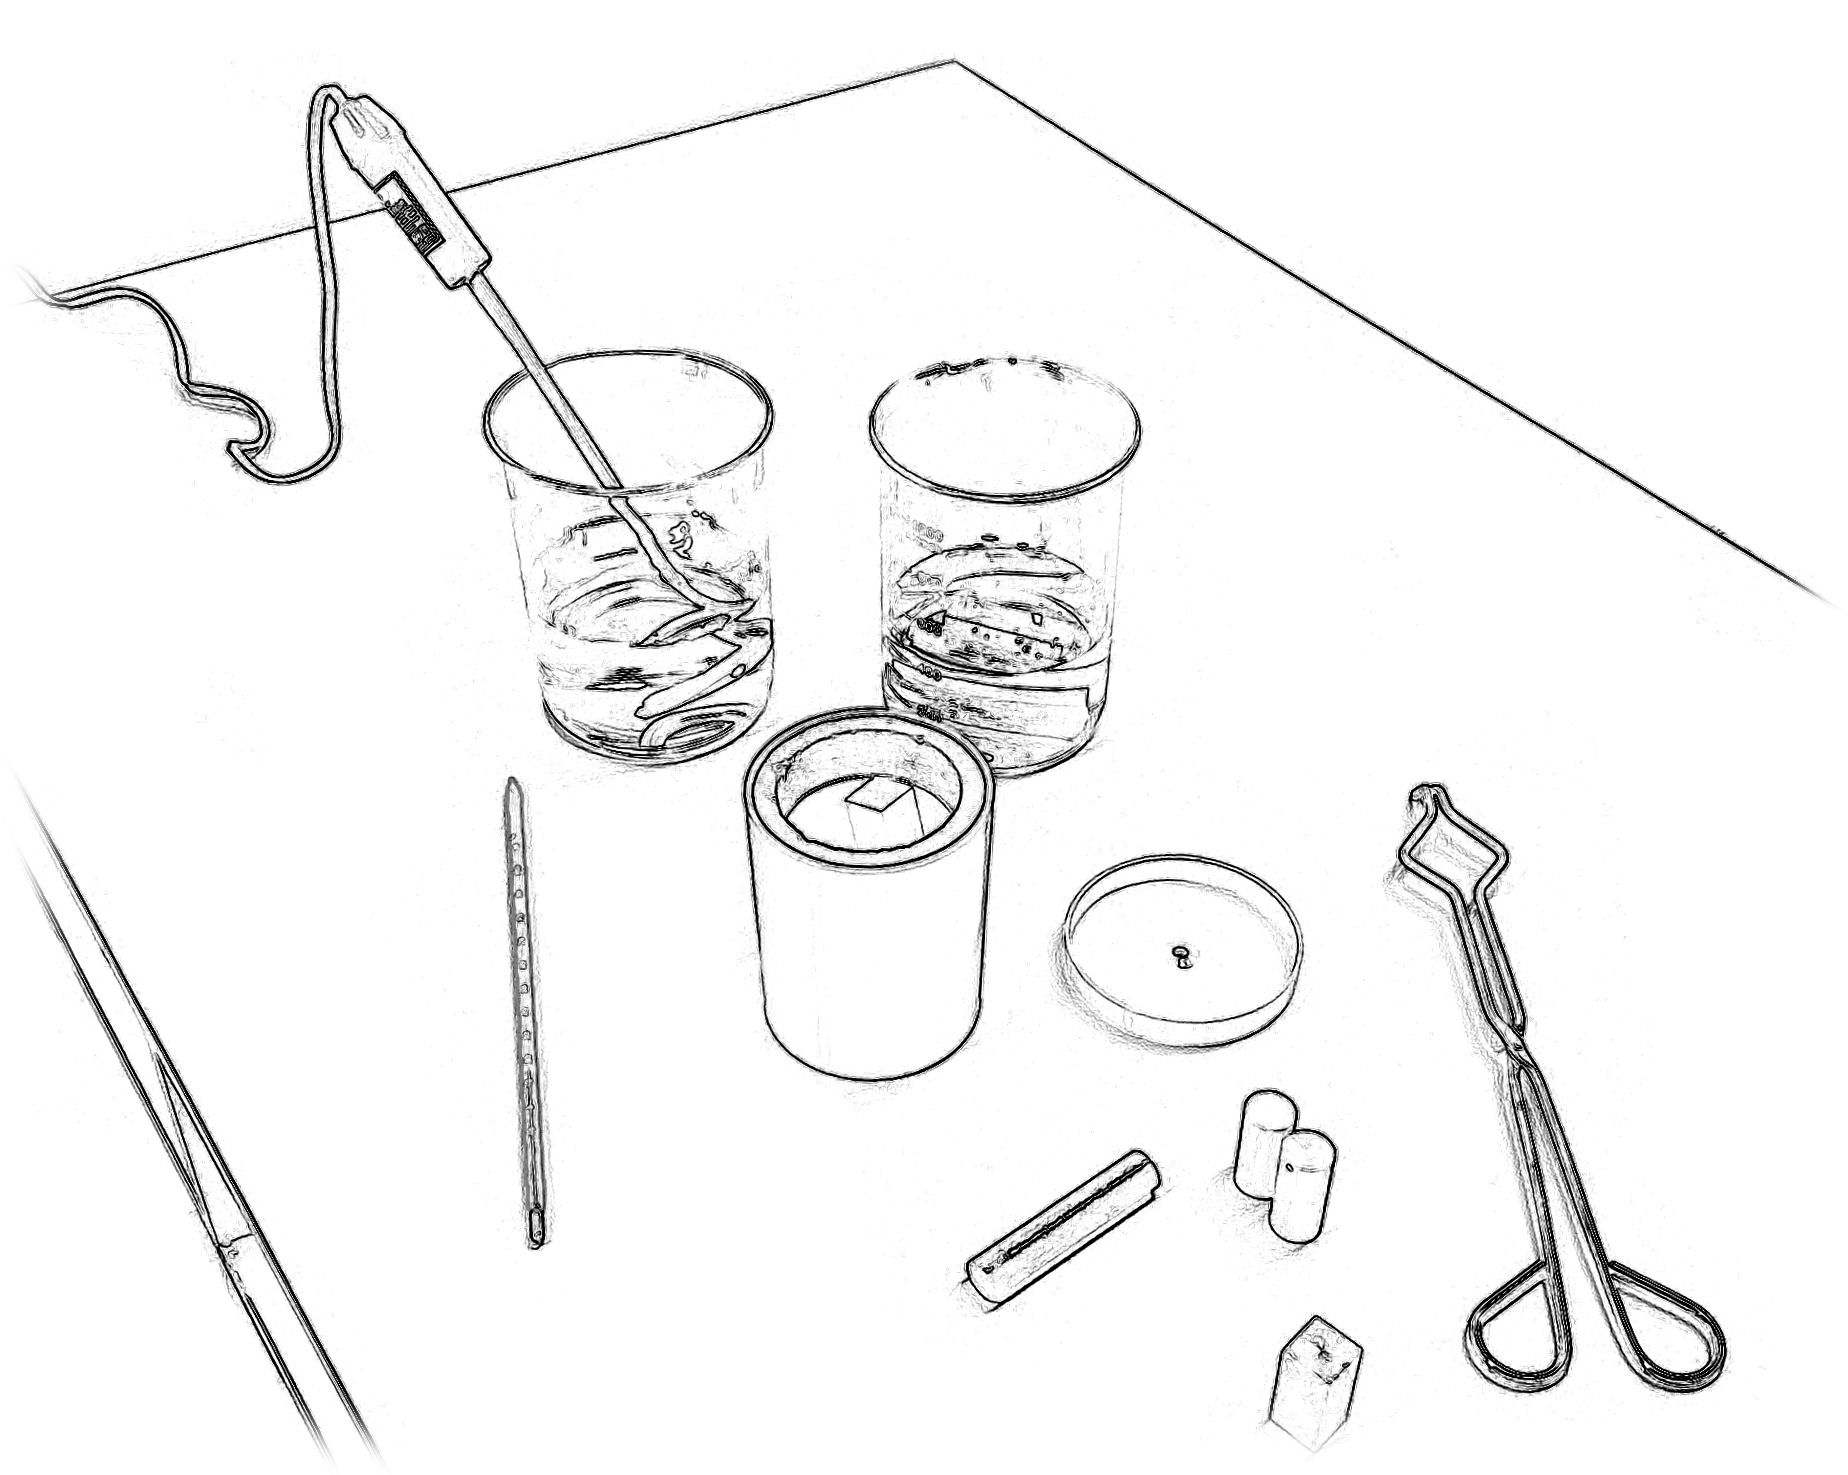
\includegraphics[width=0.7\textwidth]{Ilustrations/AparatoCalorEspecifico}
	\caption{Aparato para a verificação do calor específico de sólidos.}
\end{figure}

%%%%%%%%%%%%%%%%%%%%%%%%%%%%%%%%%%%%%%%%%%%%%%%%%%%%%%%%%%%%%%%%%%%%%%%%%%%%%%%
\section{Procedimento Experimental}
%%%%%%%%%%%%%%%%%%%%%%%%%%%%%%%%%%%%%%%%%%%%%%%%%%%%%%%%%%%%%%%%%%%%%%%%%%%%%%%

%%%%%%%%%%%%%%%%%%%%%
\subsection{Determinação da Capacidade Térmica do Calorímetro} % Se necessário
%%%%%%%%%%%%%%%%%%%%%
\begin{enumerate}
	\item Determine a massa $m^{\text{Cal}}$ do calorímetro com o auxílio da balança, anote o resultado na Tabela~\ref{Tab:CapacidadeTermica};
	\item Adicione água fria\footnote{Aqui ``água fria'' se refere a água a qualquer temperatura significativamente menor que a temperatura da água quente utilizada. Se a temperatura da água quente for de aproximadamente \np[\tcdegree C]{100,0}, por exemplo, para os nossos propósitos podemos considerar água à temperatura ambiente como fria.} ao calorímetro até que ela cubra aproximadamente um quarto da parte metálica interna;
	\item Verifique a massa $m^{\text{Cal}}_{\text{água fria}}$ do calorímetro com a água e anote na Tabela~\ref{Tab:CapacidadeTermica};
	\item Aguarde até que o sistema entre em equilíbrio térmico. Uma vez atingido o equilíbrio, com o auxílio do termômetro, determine a temperatura inicial $T_i$ do calorímetro e a anote na Tabela~\ref{Tab:CapacidadeTermica}. A partir de agora, mantenha o calorímetro sempre tampado;
	\item Verifique a temperatura da água quente disponível e anote na Tabela~\ref{Tab:CapacidadeTermica};
	\item Imediatamente após verificar a temperatura da água quente, adicione água quente ao calorímetro até cobrir aproximadamente a metade da cuba metálica interna. Aguarde o equilíbrio e verifique a temperatura final $T_f$ do calorímetro, anotando na Tabela~\ref{Tab:CapacidadeTermica};
	\item Verifique a massa final $m^{\text{Cal}}_{\text{água fria+quente}}$ do sistema;
	\item Descarte a água do calorímetro e repita o procedimento descrito acima mais duas vezes, anotando os dados na Tabela~\ref{Tab:CapacidadeTermica}
\end{enumerate}

%%%%%%%%%%%%%%%%%%%%%%%%%%%%%%%%%%%%%%%%%%%%%%%%%%%%%%%%
\subsection{Determinação do calor específico de sólidos}
%%%%%%%%%%%%%%%%%%%%%%%%%%%%%%%%%%%%%%%%%%%%%%%%%%%%%%%%

\begin{enumerate}
	\item Determine a massa $m^{\text{Cal}}$ do calorímetro com o auxílio da balança, anote o resultado na Tabela~\ref{Tab:CalorEspecificoCorpo1};
	\item Adicione água fria ao calorímetro até que ela cubra aproximadamente um quarto da parte metálica interna;
	\item Verifique a massa $m^{\text{Cal}}_{\text{água fria}}$ do calorímetro com a água fria e anote na Tabela~\ref{Tab:CalorEspecificoCorpo1};
	\item Aguarde até que o sistema entre em equilíbrio térmico. Uma vez atingido o equilíbrio, com o auxílio do termômetro, determine a temperatura inicial $T_i$ do calorímetro e a anote na Tabela~\ref{Tab:CalorEspecificoCorpo1}. A partir de agora, mantenha o calorímetro sempre tampado;
	\item Tome um dos materiais à sua escolha\footnote{Se houver mais que uma amostra do mesmo material disponível, tome mais que uma. Quanto maior for a massa, menor será o erro na determinação do calor específico.} e o submerja na água quente. Aguarde até que a amostra entre em equilíbrio térmico com a água. Verifique a temperatura $T_{\text{amostra}}$ do banho térmico e anote na Tabela~\ref{Tab:CalorEspecificoCorpo1}.
	\item Retire a amostra do banho quente e a coloque rapidamente no calorímetro. Aguarde o equilíbrio térmico\footnote{Se as amostras forem metálicas, o equilíbrio será atingido rapidamente. Não aguarde um tempo muito longo pois nesse caso a energia térmica perdida pelo calorímetro para o ambiente será significativa.} e verifique temperatura final $T_f$ do calorímetro. Anote os resultados na Tabela~\ref{Tab:CalorEspecificoCorpo1}.
	\item Retire a amostra do calorímetro, seque-a e verifique sua massa\footnote{Caso a amostra do material seja um corpo rígido, não é necessário aferir sua massa novamente.} $m_{\text{a}}$ com o auxílio da balança e a anote na Tabela~\ref{Tab:CalorEspecificoCorpo1}.
	\item Repita o procedimento acima mais duas vezes para o mesmo material. Após finalizar os procedimentos para o material em questão, repita o procedimento para outro material, também por três vezes, anotando os resultados nas Tabelas~\ref{Tab:CalorEspecificoCorpo2} a~\ref{Tab:CalorEspecificoCorpo3}.
\end{enumerate}

%%%%%%%%%%%%%%%%%%%%%%%%%%%%%%%%%%%%%%%%%%%%%%%%%%%%%%%%%%%%%%%%%%%%%%%%%%%%%%%
%%%%%%%%%%%%%%%%%%%%%%%%%%%%%%%%%%%%%%%%%%%%%%%%%%%%%%%%%%%%%%%%%%%%%%%%%%%%%%%
%%%%%%%%%%%%%%%%%%%%%%%%%%%%%%%%%%%%%%%%%%%%%%%%%%%%%%%%%%%%%%%%%%%%%%%%%%%%%%%
%%%%%%%%%%%%%%%%%%%%%%%%%%%%%%%%%%%%%%%%%%%%%%%%%%%%%%%%%%%%%%%%%%%%%%%%%%%%%%%
\cleardoublepage

\noindent{}{\huge\textit{Calor Específico de Sólidos}}

\vspace{15mm}

\begin{fullwidth}
\noindent{}\makebox[0.6\linewidth]{Turma:\enspace\hrulefill}\makebox[0.4\textwidth]{  Data:\enspace\hrulefill}
\vspace{5mm}

\noindent{}\makebox[0.6\linewidth]{Aluno(a):\enspace\hrulefill}\makebox[0.4\textwidth]{  Matrícula:\enspace\hrulefill}

\noindent{}\makebox[0.6\linewidth]{Aluno(a):\enspace\hrulefill}\makebox[0.4\textwidth]{  Matrícula:\enspace\hrulefill}

\noindent{}\makebox[0.6\linewidth]{Aluno(a):\enspace\hrulefill}\makebox[0.4\textwidth]{  Matrícula:\enspace\hrulefill}

\noindent{}\makebox[0.6\linewidth]{Aluno(a):\enspace\hrulefill}\makebox[0.4\textwidth]{  Matrícula:\enspace\hrulefill}

\noindent{}\makebox[0.6\linewidth]{Aluno(a):\enspace\hrulefill}\makebox[0.4\textwidth]{  Matrícula:\enspace\hrulefill}
\end{fullwidth}

\vspace{5mm}

%%%%%%%%%%%%%%%%%%%%%%%%%%%%%%%%%%%%%%%%%%%%%%%%%%%%%%%%%%%%%%%%%%%%%%%%%%%%%%%
\section{Questionário}
%%%%%%%%%%%%%%%%%%%%%%%%%%%%%%%%%%%%%%%%%%%%%%%%%%%%%%%%%%%%%%%%%%%%%%%%%%%%%%%

\begin{question}[type={exam}]{1}
Liste os instrumentos de medida utilizados. Descreva o tipo do equipamento, sua resolução, e seu erro de escala.
\end{question}

\begin{question}[type={exam}]{2}
Preencha as tabelas com o número adequado de algarismos significativos, unidades, e erros de escala apropriados. 
\end{question}

\begin{question}[type={exam}]{2}
Calcule a capacidade térmica do calorímetro, juntamente com o erro propagado, para as três medidas realizadas. Obtenha o valor médio e o erro associado. Apresente os cálculos realizados.
\end{question}

\begin{question}[type={exam}]{3}
\begin{enumerate}[label=\roman*.]
\item Utilizando o resultado para a capacidade térmica do calorímetro e o erro associado a tal medida, calcule os calores específicos dos materiais, incluindo o erro propagado, para cada uma das três medidas de cada material. Obtenha o valor médio e o erro propagado para cada material. Apresente os cálculos realizados.

\item Identifique o material e compare o resultado obtido para o calor específico com os valores de referência na Tabela~\ref{Tab:CaloresEspecificosDeReferencia}. Calcule os erros percentuais utilizando
\begin{equation}
	E_{\%} = \left|\frac{x-x_{\text{ref}}}{x_{\text{ref}}}\right| \times 100.
\end{equation}
\end{enumerate}
\end{question}

\begin{question}[type={exam}]{2}
Considerando os objetivos do experimento, listados na Seção~\ref{Sec:ObjetivosCalorEspecifico}, e os resultados obtidos nas questões anteriores, discuta quais objetivos foram atingidos com sucesso, justificando suas conclusões. Se algum objetivo não foi atingido, discuta quais são os possíveis motivos do insucessods e que providências podem ser tomadas para que eles sejam alcançados.
\end{question}

\vfill
%%%%%%%%%%%%%%%%%%%%%%%%%%%%%%%%%%%%%%%%%%%%%%%%%%%%%%%%%%%%%%%%%%%%%%%%%%%%%%%
\pagebreak
\section{Tabelas}
%%%%%%%%%%%%%%%%%%%%%%%%%%%%%%%%%%%%%%%%%%%%%%%%%%%%%%%%%%%%%%%%%%%%%%%%%%%%%%%

\begin{table*}[!ht]
\centering
	\begin{tabular}{lp{22mm}p{22mm}p{22mm}lp{22mm}p{22mm}l}
		\toprule
		&\multicolumn{5}{l}{\textbf{Determinação da Capacidade Térmica do calorímetro}}\\
		\\
		\cmidrule{2-7}
		& Massas & \\
		\cmidrule{2-7}
		& $m^{\text{Cal}}$ & $m^{\text{Cal}}_{\text{água fria}}$ & $m^{\text{Cal}}_{\text{água fria+quente}}$ & & $m_{\text{fria}}^{\text{água}}$ & $m_{\text{quente}}^{\text{água}}$ & \\
		\cmidrule{2-4}\cmidrule{6-7}
		& \cellcolor[gray]{0.95} & \cellcolor[gray]{0.97} & \cellcolor[gray]{0.95} & & \cellcolor[gray]{0.95} & \cellcolor[gray]{0.97} & \\
		& \cellcolor[gray]{0.89} & \cellcolor[gray]{0.92} & \cellcolor[gray]{0.89} & & \cellcolor[gray]{0.89} & \cellcolor[gray]{0.92} & \\
		& \cellcolor[gray]{0.95} & \cellcolor[gray]{0.97} & \cellcolor[gray]{0.95} & & \cellcolor[gray]{0.95} & \cellcolor[gray]{0.97} & \\
		\cmidrule{2-7}
		\\
		& Temperaturas \\
		\cmidrule{2-7}
		& $T_{i}$ & $T^{\text{água}}_{\text{quente}}$ & $T_{f}$ & & $T_f - T_i$ & $T_f - T^{\text{água}}_{\text{quente}}$ \\
		\cmidrule{2-4} \cmidrule{6-7}
		& \cellcolor[gray]{0.95} & \cellcolor[gray]{0.97} & \cellcolor[gray]{0.95} & & \cellcolor[gray]{0.95} & \cellcolor[gray]{0.97} & \\
		& \cellcolor[gray]{0.89} & \cellcolor[gray]{0.92} & \cellcolor[gray]{0.89} & & \cellcolor[gray]{0.89} & \cellcolor[gray]{0.92} & \\
        & \cellcolor[gray]{0.95} & \cellcolor[gray]{0.97} & \cellcolor[gray]{0.95} & & \cellcolor[gray]{0.95} & \cellcolor[gray]{0.97} & \\
		\cmidrule{2-7}
		\bottomrule
	\end{tabular}
	\caption[][0.5cm]{Dados para o cálculo da capacidade térmica do calorímetro.}
	\label{Tab:CapacidadeTermica}
\end{table*}
\vspace{2cm}
\begin{table*}[!ht]\forceversofloat
\centering
	\begin{tabular}{lp{22mm}p{22mm}p{22mm}lp{22mm}p{22mm}l}
		\toprule
        \multicolumn{6}{l}{\textbf{Determinação do Calor Específico, Material N\textordmasculine~1}}\\
        \\
		& Massas \\
		\cmidrule{2-6}
		& $m^{\text{Cal}}$ & $m^{\text{Cal}}_{\text{água fria}}$ & $m_{\text{a}}$ & & $m_{\text{fria}}^{\text{água}}$ & \\
		\cmidrule{2-4} \cmidrule{6-6}
		& \cellcolor[gray]{0.95} & \cellcolor[gray]{0.97} & \cellcolor[gray]{0.95} & & \cellcolor[gray]{0.95} & \\
		& \cellcolor[gray]{0.89} & \cellcolor[gray]{0.92} & \cellcolor[gray]{0.89} & & \cellcolor[gray]{0.89} & \\
		& \cellcolor[gray]{0.95} & \cellcolor[gray]{0.97} & \cellcolor[gray]{0.95} & & \cellcolor[gray]{0.95} & \\
		\cmidrule{2-6}
		\\
		& Temperaturas \\
		\cmidrule{2-4}\cmidrule{6-7}
		& $T_{i}$ & $T_{\text{amostra}}$ & $T_{f}$ & & $T_f - T_i$ & $T_f - T_{\text{amostra}}$ & \\
		\cmidrule{2-4}\cmidrule{6-7}
		& \cellcolor[gray]{0.95} & \cellcolor[gray]{0.97} & \cellcolor[gray]{0.95} & & \cellcolor[gray]{0.95} & \cellcolor[gray]{0.97} & \\
		& \cellcolor[gray]{0.89} & \cellcolor[gray]{0.92} & \cellcolor[gray]{0.89} & & \cellcolor[gray]{0.89} & \cellcolor[gray]{0.92} & \\
		& \cellcolor[gray]{0.95} & \cellcolor[gray]{0.97} & \cellcolor[gray]{0.95} & & \cellcolor[gray]{0.95} & \cellcolor[gray]{0.97} & \\
		\cmidrule{2-7}
		\bottomrule
	\end{tabular}
	\caption[][0.5cm]{Dados para o cálculo do calor específico.}
	\label{Tab:CalorEspecificoCorpo1}
\end{table*}
\vfill
\pagebreak

\begin{table*}[!ht]\forcerectofloat
\centering
	\begin{tabular}{lp{22mm}p{22mm}p{22mm}lp{22mm}p{22mm}l}
		\toprule
        \multicolumn{6}{l}{\textbf{Determinação do Calor Específico, Material N\textordmasculine~2}}\\
        \\
		& Massas \\
		\cmidrule{2-6}
		& $m^{\text{Cal}}$ & $m^{\text{Cal}}_{\text{água fria}}$ & $m_{\text{a}}$ & & $m_{\text{fria}}^{\text{água}}$ & \\
		\cmidrule{2-4} \cmidrule{6-6}
		& \cellcolor[gray]{0.95} & \cellcolor[gray]{0.97} & \cellcolor[gray]{0.95} & & \cellcolor[gray]{0.95} & \\
		& \cellcolor[gray]{0.89} & \cellcolor[gray]{0.92} & \cellcolor[gray]{0.89} & & \cellcolor[gray]{0.89} & \\
		& \cellcolor[gray]{0.95} & \cellcolor[gray]{0.97} & \cellcolor[gray]{0.95} & & \cellcolor[gray]{0.95} & \\
		\cmidrule{2-6}
		\\
		& Temperaturas \\
		\cmidrule{2-4}\cmidrule{6-7}
		& $T_{i}$ & $T_{\text{amostra}}$ & $T_{f}$ & & $T_f - T_i$ & $T_f - T_{\text{amostra}}$ & \\
		\cmidrule{2-4}\cmidrule{6-7}
		& \cellcolor[gray]{0.95} & \cellcolor[gray]{0.97} & \cellcolor[gray]{0.95} & & \cellcolor[gray]{0.95} & \cellcolor[gray]{0.97} & \\
		& \cellcolor[gray]{0.89} & \cellcolor[gray]{0.92} & \cellcolor[gray]{0.89} & & \cellcolor[gray]{0.89} & \cellcolor[gray]{0.92} & \\
		& \cellcolor[gray]{0.95} & \cellcolor[gray]{0.97} & \cellcolor[gray]{0.95} & & \cellcolor[gray]{0.95} & \cellcolor[gray]{0.97} & \\
		\cmidrule{2-7}
		\bottomrule
	\end{tabular}
	\caption[][0.5cm]{Dados para o cálculo do calor específico.}
	\label{Tab:CalorEspecificoCorpo2}
\end{table*}
\vfill


